\documentclass{beamer}
%\usetheme{Ilmenau}
%\usecolortheme{beaver}

\usepackage[slovak,american]{babel}
\usepackage[utf8]{inputenc}
\usepackage{graphicx}
\usepackage{adjustbox}

 \usepackage{xcolor}
 
 \newsavebox\MBox
\newcommand\Cline[2][red]{{\sbox\MBox{$#2$}%
  \rlap{\usebox\MBox}\color{#1}\rule[-2.2\dp\MBox]{\wd\MBox}{1pt}}}

%\usefonttheme{serif}

%\definecolor{UKOrange}{HTML}{ef9424} %
\definecolor{UKOrange}{HTML}{7a2c18} %
\definecolor{UKBrown}{HTML}{a96d5e} %
\definecolor{UKLight}{HTML}{d8b6ab} %
\definecolor{UKDark}{HTML}{7a4f44}
\definecolor{UKDarker}{HTML}{4d312b} 
\definecolor{UKDarkest}{HTML}{2e1e1a}
\definecolor{UKRed}{HTML}{bf1f1c}

\setbeamertemplate{footline}[frame number]{}
\setbeamertemplate{navigation symbols}{}

%\usecolortheme{beaver}
\setbeamertemplate{itemize item}[square]
\setbeamercolor{itemize item}{fg = UKBrown}
\setbeamercolor{itemize subitem}{fg = UKLight}
\setbeamercolor{enumerate item}{fg = UKDark}

\setbeamercolor{footnote}{fg=UKLight}
\setbeamercolor{footnote mark}{fg=UKLight}
\setbeamerfont{footnote}{size=\tiny}
\renewcommand\footnoterule{}

\usetheme{default}
\beamertemplatenavigationsymbolsempty
\setbeamercolor{title}{fg=white, bg=UKBrown}
\setbeamercolor{frametitle}{fg=white, bg=UKBrown}
\setbeamercolor{block title}{bg=UKBrown, fg= white}
\setbeamercolor{block body}{bg =UKLight, fg = UKDarkest}

\setbeamercolor{block title alerted}{bg=UKOrange, fg= white}
\setbeamercolor{block body alerted}{bg =UKLight, fg = UKDarkest}


%\setbeamercolor{section in toc}{fg = UKBrown}
%\setbeamercolor{section in toc}{fg = UKDarkest}

% odstrani gulicky
\renewcommand*{\slideentry}[6]{}

\useoutertheme[subsection=false]{miniframes}
\AtBeginSection[]{\subsection{}}

\setbeamercolor{below lower separation line head}{bg=UKDark}
\addtobeamertemplate{headline}{}{%
  \begin{beamercolorbox}[colsep=0.5pt]{below lower separation line head}
  \end{beamercolorbox}
}
%\setbeamercolor*{mini frame}{fg=white,bg=UKRosy}
\setbeamercolor{section in head/foot}{fg=UKLight, bg=UKDark}

\usepackage{etoolbox}
\makeatletter
\preto{\@verbatim}{\topsep=0pt \partopsep=0pt }
\makeatother

%\setbeamertemplate{itemize/enumerate body begin}{\normalsize}
%\setbeamertemplate{itemize/enumerate subbody begin}{\normalsize}




%\newcommand{\codeblock}[2]{ \begin{block}{#1} \begin{verbatim}#2\end{verbatim}\end{block}}

%\defbeamertemplate*{title page}{customized}[1][]
%{
%  \begin{centering}
%    \begin{beamercolorbox}[sep=8pt,center]{title}
%      \usebeamerfont{title}\inserttitle
%    \end{beamercolorbox}
%  \end{centering}
%  \bigskip
%
%\begin{columns}[onlytextwidth,T]
%
%
%  \column{27mm}
%  \includegraphics[width=27mm]{images/logoFMFI.png}
%  
%  \column{\dimexpr\linewidth-54mm-6mm}
%  \centering
%  \vspace{5mm}  
%  \usebeamerfont{author}\insertauthor\par
%  \vspace{5mm}
%  \usebeamerfont{institute}\insertinstitute\par
%
%  \column{27mm}
%  \includegraphics[width=27mm]{images/logoUK.png}  
%\end{columns}
%\centering
%\vspace{7mm}
%  \usebeamerfont{date}\insertdate\par
%}

\DeclareMathOperator*{\argmin}{arg\,min}
\newcommand{\e}[1]{$\cdot 10^{#1}$}
\newcommand*\mean[1]{\bar{#1}}

\newcommand*{\Z}{\mathbb{Z}}

%\newcommand{\codeblock}[2]{ \begin{block}{#1} \begin{verbatim}#2\end{verbatim}\end{block}}



\title[8. cvičenie]{Pokročilé spracovanie obrazu - Morfológia II.}
\author[Kocur]{Ing. Viktor Kocur \\{\small viktor.kocur@fmph.uniba.sk}}
\institute{DAI FMFI UK}
\date{13.11.2018}

\begin{document}
\selectlanguage{slovak}

\begin{frame}
  \titlepage
\end{frame}

\section{Binárne obrazy}
\subsection{Granulometria}

\begin{frame}
\frametitle{Granulometria}
  \begin{block}{Opening with various SE}
  If we open a binary image with consecutively bigger structural elements we can retrieve information about the distribution of the object sizes.
  \end{block}
  

  \begin{block}{Exercise}
  Open the image granulometria.png with consecutively bigger structural elements. Display a bar graph showing the relationship between the area of the opened image and the size of the SE.
  \end{block}
\end{frame}

\subsection{Conditional dilation}

\begin{frame}
\frametitle{Conditional dilation}
  \begin{block}{Conditional dilation - definition}
  The image is thresholded with two different thresholds. We thus obtain two images: $A$ for the higher threshold and $B$ for the lower one. Conditional dilation with structural element $SE$ is defined as: $(A \oplus SE) \cap B$.
  \end{block}  

  \begin{block}{Exercise}
  Test the conditional dilation for the image bunky.png.
  \end{block}
\end{frame}

\section{Grayscale morphology}

\subsection{Morphological operations}

\begin{frame}
\frametitle{Grayscale erosion and dilation} 

  \begin{block}{Dilation and erosion}
  For $f, h \colon \mathbb{R}^2 \to \mathbb{R}$ with finite support we define: \\ $f \oplus h = max\{ f(x-r, y-s) + h (r,s) | (r,s) \in supp(h)\}$ and \\
  $f \ominus h = min\{ f(x-r, y-s) - h (r,s) | (r,s) \in supp(h)\}$
  \end{block}   

  \begin{block}{Matlab}
  Function names in Matlab are the same as function names for binary images.
  \end{block}
  
  \begin{block}{Úloha}
  Test dilation, erosion, opening and closing on the image zatisie.pgm. Use closing and subsequent opening to smooth the image.
  \end{block}   
\end{frame}


\subsection{Morphological gradient}

\begin{frame}
\frametitle{Morphological gradient} 

  \begin{block}{Morphological gradient}
  $grad(I) = \frac{(I \oplus SE) - (I \ominus SE)}{2}$
  \end{block}   

  \begin{block}{Morphological gradient - internal}
  $grad(I) = I - (I \ominus SE)$
  \end{block}     
  
  \begin{block}{Morphological gradient - external}
  $grad(I) = (I \oplus SE) - I$
  \end{block}     
  
  \begin{block}{Úloha}
  Otestujte detekciu hrán pomocou morfologického gradientu.
  \end{block}   
\end{frame}

\subsection{Top and Bottom-hat}

\begin{frame}
\frametitle{Top-hat and bottom-hat transformation} 

  \begin{block}{Top-hat transformation}
  Top-hat transformation is the difference of the original image and its opening. Bottom-hat transformation is the difference of the closing of an image and its original.
  \end{block}  
  
  \begin{block}{imtophat}
  imtophat(I, SE) - returns top-hat transformation of the image with structural element SE
  \end{block}    
  
  \begin{block}{imbothat}
  imbothat(I, SE) - returns top-hat transformation of the image with structural element SE
  \end{block}      
\end{frame}

\begin{frame}
\frametitle{Adaptive segmentation} 

  \begin{block}{Segmenting on non-constant background}
  We can utilize the top-hat transformation to segment light objects on non-constant background. Bottom-hat can be used to segment dark objects.
  \end{block}  
  
  \begin{block}{Exercise}
  Segment the qr codes in qr.png and rice from rice.png (included in Matlab)
  \end{block}    
\end{frame}

\begin{frame}
\frametitle{Contrast correction} 
  \begin{block}{Increasing contrast}
  We can increase the image contrast by adding the top-hat transformation and subtracting the bottom-hat transformation from the original.
  \end{block} 
  
  \begin{block}{Exercise}
  Increase contrast in krajinka.png
  \end{block}          
\end{frame}

\subsection{Reconstruction}

\begin{frame}
\frametitle{Reconstruction}
\begin{center}
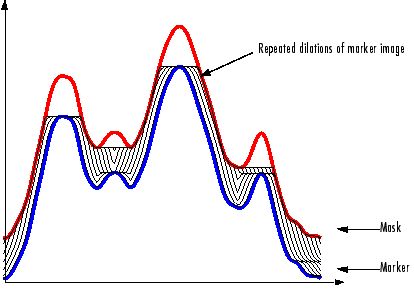
\includegraphics[width= 0.8\textwidth]{recon.png}
\end{center}
\end{frame}


\begin{frame}
\frametitle{Reconstruction}
\begin{center}
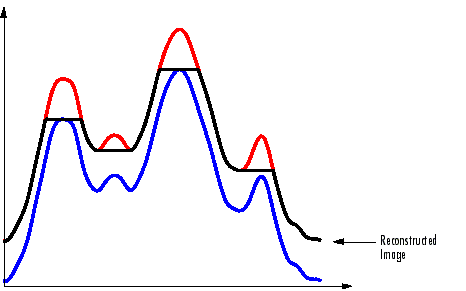
\includegraphics[width= 0.8\textwidth]{recon2.png}
\end{center}
\end{frame}

\begin{frame}
\frametitle{Reconstruction}

  \begin{block}{Filling a chosen object}
  We can use reconstruction to segment chosen objects in a binary image. To do this we choose a marker in a way which contains only the points that are in the object we want to segment.

  \end{block}  
  
  \begin{block}{imreconstruct}
  imreconstruct(marker, mask) - returns reconstruction of mask by the given marker.
  \end{block}  
  
  \begin{block}{Exercise}
  Use ginput and segment only the letter in text.png which gets clicked on by the user.
  \end{block}  
\end{frame}



\end{document}